% This file was created with tikzplotlib v0.10.1.
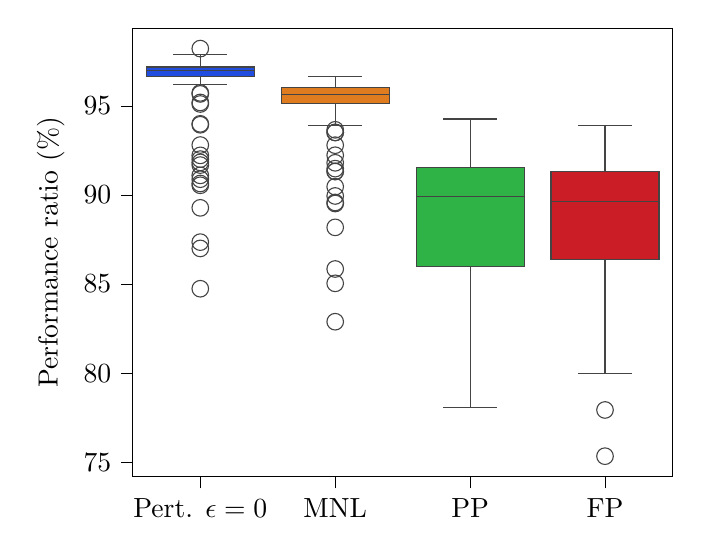
\begin{tikzpicture}

\definecolor{chocolate22312431}{RGB}{223,124,31}
\definecolor{darkgray176}{RGB}{176,176,176}
\definecolor{darkslategray68}{RGB}{68,68,68}
\definecolor{firebrick2032937}{RGB}{203,29,37}
\definecolor{limegreen4717970}{RGB}{47,179,70}
\definecolor{royalblue3378223}{RGB}{33,78,223}

\begin{axis}[
tick align=outside,
tick pos=left,
x grid style={darkgray176},
xmin=-0.5, xmax=3.5,
xtick style={color=black},
xtick={0,1,2,3},
xticklabels={Pert. \(\displaystyle \epsilon=0\),MNL,PP,FP},
y grid style={darkgray176},
ylabel={Performance ratio (\%)},
ymin=74.1910997484927, ymax=99.361593772276,
ytick style={color=black},
ytick={70,75,80,85,90,95,100},
yticklabels={
  \(\displaystyle {70}\),
  \(\displaystyle {75}\),
  \(\displaystyle {80}\),
  \(\displaystyle {85}\),
  \(\displaystyle {90}\),
  \(\displaystyle {95}\),
  \(\displaystyle {100}\)
}
]
\path [draw=darkslategray68, fill=royalblue3378223]
(axis cs:-0.4,96.6419615346797)
--(axis cs:0.4,96.6419615346797)
--(axis cs:0.4,97.1868975892247)
--(axis cs:-0.4,97.1868975892247)
--(axis cs:-0.4,96.6419615346797)
--cycle;
\addplot [darkslategray68]
table {%
0 96.6419615346797
0 96.2165776607347
};
\addplot [darkslategray68]
table {%
0 97.1868975892247
0 97.9052317733693
};
\addplot [darkslategray68]
table {%
-0.2 96.2165776607347
0.2 96.2165776607347
};
\addplot [darkslategray68]
table {%
-0.2 97.9052317733693
0.2 97.9052317733693
};
\addplot [black, mark=o, mark size=3, mark options={solid,fill opacity=0,draw=darkslategray68}, only marks]
table {%
0 91.8279480049551
0 84.7358075575047
0 95.731481858829
0 87.3523052390947
0 90.8844376264629
0 91.6782689356234
0 92.8037957744955
0 90.5444487946375
0 89.2767045807754
0 95.6738294834345
0 86.9985047098216
0 90.6443018209354
0 92.2229984354157
0 92.0129322350107
0 95.1941046744618
0 93.9416729650652
0 91.1006434706477
0 95.1077941488231
0 93.9942138781203
0 98.2174804075586
};
\path [draw=darkslategray68, fill=chocolate22312431]
(axis cs:0.6,95.110363317606)
--(axis cs:1.4,95.110363317606)
--(axis cs:1.4,96.0240261224948)
--(axis cs:0.6,96.0240261224948)
--(axis cs:0.6,95.110363317606)
--cycle;
\addplot [darkslategray68]
table {%
1 95.110363317606
1 93.8924768411228
};
\addplot [darkslategray68]
table {%
1 96.0240261224948
1 96.6358324586154
};
\addplot [darkslategray68]
table {%
0.8 93.8924768411228
1.2 93.8924768411228
};
\addplot [darkslategray68]
table {%
0.8 96.6358324586154
1.2 96.6358324586154
};
\addplot [black, mark=o, mark size=3, mark options={solid,fill opacity=0,draw=darkslategray68}, only marks]
table {%
1 82.8842530770368
1 89.5204426414265
1 90.4651890543327
1 91.4780454323682
1 89.5787084160496
1 88.180842255625
1 85.8443944298772
1 91.8057237139984
1 91.3251492021376
1 93.5077074695329
1 93.6575289638538
1 92.2301017442514
1 89.9438044704687
1 93.5124748810001
1 85.0386548103656
1 91.3128459352645
1 92.7947374136883
};
\path [draw=darkslategray68, fill=limegreen4717970]
(axis cs:1.6,85.9939607721336)
--(axis cs:2.4,85.9939607721336)
--(axis cs:2.4,91.5599409422826)
--(axis cs:1.6,91.5599409422826)
--(axis cs:1.6,85.9939607721336)
--cycle;
\addplot [darkslategray68]
table {%
2 85.9939607721336
2 78.0485963504318
};
\addplot [darkslategray68]
table {%
2 91.5599409422826
2 94.26559936098
};
\addplot [darkslategray68]
table {%
1.8 78.0485963504318
2.2 78.0485963504318
};
\addplot [darkslategray68]
table {%
1.8 94.26559936098
2.2 94.26559936098
};
\path [draw=darkslategray68, fill=firebrick2032937]
(axis cs:2.6,86.358498706691)
--(axis cs:3.4,86.358498706691)
--(axis cs:3.4,91.3063709310569)
--(axis cs:2.6,91.3063709310569)
--(axis cs:2.6,86.358498706691)
--cycle;
\addplot [darkslategray68]
table {%
3 86.358498706691
3 79.9520251212715
};
\addplot [darkslategray68]
table {%
3 91.3063709310569
3 93.9166913358089
};
\addplot [darkslategray68]
table {%
2.8 79.9520251212715
3.2 79.9520251212715
};
\addplot [darkslategray68]
table {%
2.8 93.9166913358089
3.2 93.9166913358089
};
\addplot [black, mark=o, mark size=3, mark options={solid,fill opacity=0,draw=darkslategray68}, only marks]
table {%
3 75.3352131132101
3 77.9293968694246
};
\addplot [darkslategray68]
table {%
-0.4 96.9900443614698
0.4 96.9900443614698
};
\addplot [darkslategray68]
table {%
0.6 95.6474432911195
1.4 95.6474432911195
};
\addplot [darkslategray68]
table {%
1.6 89.9159767633996
2.4 89.9159767633996
};
\addplot [darkslategray68]
table {%
2.6 89.6544379872342
3.4 89.6544379872342
};
\draw (axis cs:0,67.8984762425468) node[
  scale=0.75,
  anchor=base,
  text=black,
  rotate=0.0
]{\bfseries 96.19};
\draw (axis cs:1,67.8984762425468) node[
  scale=0.75,
  anchor=base,
  text=black,
  rotate=0.0
]{\bfseries 94.90};
\draw (axis cs:2,67.8984762425468) node[
  scale=0.75,
  anchor=base,
  text=black,
  rotate=0.0
]{\bfseries 88.64};
\draw (axis cs:3,67.8984762425468) node[
  scale=0.75,
  anchor=base,
  text=black,
  rotate=0.0
]{\bfseries 88.58};
\draw (axis cs:-1,68.1501811827847) node[
  scale=0.75,
  text=black,
  rotate=0.0
]{\bfseries \textbf{Average:}};
\end{axis}

\end{tikzpicture}
